\documentclass[letterpaper, 8pt]{extarticle}
\usepackage{amssymb,amsmath,amsthm,amsfonts}
\usepackage{multicol,multirow}
\usepackage{calc}
\usepackage{ifthen}
\usepackage[landscape]{geometry}
\usepackage[colorlinks=true,citecolor=blue,linkcolor=blue]{hyperref}

\usepackage{booktabs}
\usepackage{ulem}
\usepackage{enumitem}
\usepackage{tabulary}
\usepackage{graphicx}
\usepackage{siunitx}
\usepackage{tikz}
\usepackage{derivative}
\usepackage{svg}
\usepackage{listings}
\usepackage{setspace}
\usepackage{listings}
\usepackage{xcolor}
\usepackage{courier}
\usepackage{syntax}
\usepackage{mathpartir}
\usepackage{braket}

% minimal line spacing
% \setstretch{0.1}

% set borders (experimentally determined to minimize cutoff and maximize space on school printers)
\geometry{top=.25in,left=.25in,right=.25in,bottom=.35in}

% make figures work better in multicol
% \newenvironment{Figure}
% {\par\medskip\noindent\minipage}
% {\endminipage\par\medskip}

% \pagestyle{empty} % clear page

% rewrite section commands to be smaller
\makeatletter
\renewcommand{\section}{\@startsection{section}{1}{0mm}%
                                {-1explus -.5ex minus -.2ex}%
                                {0.5ex plus .2ex}%x
                                {\normalfont\normalsize\bfseries}}
\renewcommand{\subsection}{\@startsection{subsection}{2}{0mm}%
                                {-1explus -.5ex minus -.2ex}%
                                {0.5ex plus .2ex}%
                                {\normalfont\small\bfseries}}
\renewcommand{\subsubsection}{\@startsection{subsubsection}{3}{0mm}%
                                {-1ex plus -.5ex minus -.2ex}%
                                {1ex plus .2ex}%
                                {\normalfont\tiny\bfseries}}
\makeatother
\setcounter{secnumdepth}{0} % disable section numbering


% disable indenting
\setlength{\parindent}{0pt}
\setlength{\parskip}{0pt plus 0.5ex}

% Custom siunitx defs
\DeclareSIUnit\noop{\relax}
\NewDocumentCommand\prefixvalue{m}{%
\qty[prefix-mode=extract-exponent,print-unity-mantissa=false]{1}{#1\noop}
}

% Shorthand definitions
\newcommand{\To}{\Rightarrow}
\newcommand{\ttt}{\texttt}
\newcommand{\ra}{\rightarrow}

% condense itemize & enumerate
\let\olditemize=\itemize \let\endolditemize=\enditemize \renewenvironment{itemize}{\olditemize \itemsep0em}{\endolditemize}
\let\oldenumerate=\enumerate \let\endoldenumerate=\endenumerate \renewenvironment{enumerate}{\oldenumerate \itemsep0em}{\endoldenumerate}
\setlist[itemize]{noitemsep, topsep=0pt, leftmargin=*}
\setlist[enumerate]{noitemsep, topsep=0pt, leftmargin=*}

\title{3QI3}

\begin{document}
\raggedright
\tiny

% make listings look nicer
% \lstset{
%     tabsize = 2, %% set tab space width
%     showstringspaces = false, %% prevent space marking in strings, string is defined as the text that is generally printed directly to the console
%     basicstyle = \tiny\ttfamily, %% set listing font and size
%     breaklines = true, %% enable line breaking
%     numberstyle = \tiny,
%     postbreak = \mbox{\textcolor{red}{\(\hookrightarrow\)}\space}
% }

\begin{center}
    {\textbf{Physics 3QI3 - Key Exchange Edition}} \\
\end{center}
% set column spacing rules
\setlength{\premulticols}{1pt}
\setlength{\postmulticols}{1pt}
\setlength{\multicolsep}{1pt}
\setlength{\columnsep}{2pt}
\begin{multicols*}{5}
    \section{Linalg}
    Matrix Multiplication:
    \(
    \begin{pmatrix}
        a & b \\
        c & d
    \end{pmatrix}
    \begin{pmatrix}
        e & f \\
        g & h
    \end{pmatrix}
    =
    \begin{pmatrix}
        ae+bg & af+bh \\
        ce+dg & cf+dh
    \end{pmatrix}
    \)

    \textbf{Adjoint (Hermitian Conjugate):}
    \(A^\dagger = A^*\)
    (transpose the matrix and take the complex conjugate of each element)

    \textbf{Complex Conjugate:}
    Flip the sign of the imaginary part of a complex number

    \textbf{Trace}
    Sum the diagonal elements of a square matrix

    \textbf{Multi-bit Dirac Notation}
    \(\ket{A} \ket{B} = \ket{AB}\)
    The dual of this is \(\bra{BA}\)

    \textbf{Properties}
    \(\ket{A}\bra{A} = \hat{I}\)

    \section{Probability and Bayes' Rule}
    \textbf{Bayes' theorem formula:}
    \[
        P(A|B) = \frac{P(B|A)P(A)}{P(B)}
    \]

    Examples of calculating conditional probabilities (medical tests, particle detectors)

    \textbf{Poisson distribution:}
    \[
        P(n) = \frac{\lambda^n e^{-\lambda}}{n!}
    \]

    \section{Classical Information Theory}
    \subsection{Shannon Entropy/Information}
    \(H = - k \sum_i p(a_i) \log p(a_i)\)
    By convention, we use \(k = 1\) and \(\log\) is base 2.
    \subsubsection{Properties of entropy}
    Entropy must be non-negative, and is maximized for a uniform distribution.

    \section{Thermodynamics}
    Gibbs Entropy: \(S = -k \sum p_i \log p_i\)

    \section{Communication Theory}
    \textbf{Number of Typical Messages}
    \(W \simeq 2^{N H(p)}\) where \(H(p)\) is the entropy of the message
    and \(N\) is the number of bits in the message.

    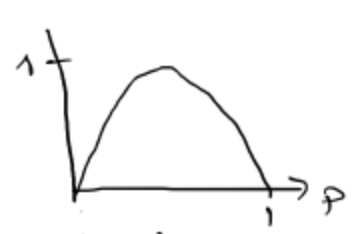
\includegraphics[width=.7\linewidth]{SCR-20240305-qtnt.png}
    Compression factor for different values of \(p\).
    As \(p\) approaches 0.5 from either side,
    we can compress the message less and less,
    since there is more entropy we need to encode.

    \subsection{Shannon's Noiseless Coding Theorem:}
    For a given message,
    we only need \(N H(p)\) bits to encode it (definition of \(H(p)\) above)

    \textbf{Example:}
    Let us have an alphabet A, B, C, D
    with probabilities of \(1/2, 1/4, 1/8, 1/8\) respectively.
    Entropy is \(H = -(1/2 \log 1/2 + 1/4 \log 1/4 \dots) = 7/4\text{ bits}\)
    Therefore, a message \(N\) characters long can be encoded in \(7/4 \cdot N\) bits.

    \subsection{Shannon's Noisy Coding Theorem:}
    On average, we need at least \(\frac{N_0}{1-H(q)}\)
    bits to encode one of \(2^{N_0}\) equally probable messages
    (\(N_0\) is the original message length)
    where \(H(q) = -[q \log q + (1-q) \log (1-q)]\)
    is the entropy associated with single bit error q.

    \textbf{Efficient Coding:}
    Plot \(N/N_0 - 1\) vs \(q\) to see when overhead becomes too ``large''

    \textbf{Huffman Coding}
    \begin{enumerate}
        \item Sort the probabilities
        \item Combine the two lowest probabilities into a tree,
              storing characters as branches and the sum of their probabilities as the root
        \item Repeat until all probabilities are combined, and we reach a probability of 1
        \item Set 0/1 to left/right (either pairing), and traverse the tree to find the encoding
    \end{enumerate}

    \section{Dirac Notation}
    \(\bra{\Psi} \Longleftrightarrow \ket{\psi}^\dagger\)

    \begin{tabular}{@{}lc@{}}\toprule
        Ket                        & Matrix                                                      \\ \midrule
        \(\ket{0}\) or \(\ket{H}\) & \(\begin{bmatrix} 1 \\ 0 \end{bmatrix}\)                    \\
        \(\ket{1}\) or \(\ket{V}\) & \(\begin{bmatrix} 0 \\ 1 \end{bmatrix}\)                    \\
        Diagonal Up                & \(\frac{1}{\sqrt{2}}\begin{bmatrix} 1 \\ 1 \end{bmatrix}\)  \\
        Diagonal Down              & \(\frac{1}{\sqrt{2}}\begin{bmatrix} 1 \\ -1 \end{bmatrix}\) \\
        Left Circular              & \(\frac{1}{\sqrt{2}}\begin{bmatrix} 1 \\ i \end{bmatrix}\)  \\
        Right Circular             & \(\frac{1}{\sqrt{2}}\begin{bmatrix} 1 \\ -i \end{bmatrix}\) \\
        \bottomrule
    \end{tabular}

    \includegraphics[width=.7\linewidth]{Bloch\_sphere.svg.png}

    \(\ket{\Psi} = \cos\frac{\theta}{2}\ket{0}+e^{i \phi}\sin\frac{\theta}{2}\ket{1}\)

    \begin{multicols*}{2}
        \(+x = \frac{1}{\sqrt{2}}(\ket{0}+\ket{1})\)
        \(-x = \frac{1}{\sqrt{2}}(\ket{0}-\ket{1})\)
        \(+y = \frac{1}{\sqrt{2}}(\ket{0}+i\ket{1})\)
        \(-y = \frac{1}{\sqrt{2}}(\ket{0}-i\ket{1})\)
    \end{multicols*}

    \textbf{Change of basis}
    Let \(\theta\) be a rotation of basis vectors,
    counterclockwise.

    \(\ket{x} = \cos\theta\ket{x'} - \sin\theta\ket{y'}\)
    and
    \(\ket{y} = \sin\theta\ket{x'} + \cos\theta\ket{y'}\)

    where \(\ket{x'}\) and \(\ket{y'}\) are the new basis vectors.

    \textbf{Outer Product}
    Given that
    \(\ket{\psi} = \)
    \(\ket{\psi}\bra{\phi} = \begin{bmatrix} \psi_1\phi_1 & \psi_1\phi_2 \\ \psi_2\phi_1 & \psi_2\phi_2 \end{bmatrix}\)

    \textbf{Quantum State Tomography}
    \begin{itemize}
        \item Set a set of observables to uniquely determine a state.
              For a single qubit, we can use the Pauli operators.
        \item Prepare many copies of the state
        \item Measure the observables and use probability and regression to reconstruct the state
    \end{itemize}

    \section{Operators}
    Operators produce another ket

    \textbf{Mean value of an observable}
    Measuring an observable
    \(\hat{V} = \sum_i v_i \ket{v_i}\bra{v_i}\)
    in the state \(\ket{\Psi}\)

    Obtains result \(v_i\) with probability
    \(p(v_i) = |\braket{v_i|\Psi}|^2\)

    Repeating measurement many times obtains \textbf{expectation value}
    \(\braket{V}=\sum_i P_i v_i = \sum_i |\braket{v_i|\Psi}|^2 v_i\)
    \(\braket{V}_\Psi = \braket{\Psi|\hat{V}|\Psi}\)

    \subsection{Uncertainty}
    Variance is
    \(
    \Delta V^2
    = \braket{\Psi|(\hat{V}-\braket{\Psi|\hat{V}|\Psi})^2|\Psi}
    \)
    \(
    \Delta V^2
    = \braket{\Psi|\hat{V}^2|\Psi} - \braket{\Psi|\hat{V}|\Psi}^2
    = \braket{\hat{V}^2}-\braket{\hat{V}}^2
    \)

    \subsection{Heisenberg Uncertainty Principle}
    \(\Delta x \Delta p \geq \frac{1}{2} |\braket{\psi | [\hat{A}, \hat{B}]| \psi}|\)
    (e.g. for \([\hat{x}, \hat{p}] = i \hbar\) we find \(\Delta x \Delta p \geq \frac{\hbar}{2}\))

    \subsection{Pauli Operators}

    \begin{tabular}{@{}l@{}} \toprule
        \(\hat{\sigma}_x
        = \begin{pmatrix}
              0 & 1 \\
              1 & 0
          \end{pmatrix}
        = \ket{0}\bra{1}+\ket{1}\bra{0}\)    \\
        \quad Eigenvectors: \(
        \begin{pmatrix}1\\0\end{pmatrix},
        \begin{pmatrix}0\\1\end{pmatrix}
        \)                                   \\
        \(\hat{\sigma}_y
        = \begin{pmatrix}
              0 & -i \\
              i & 0
          \end{pmatrix}
        = i(\ket{1}\bra{0}-\ket{0}\bra{1})\) \\
        \quad Eigenvectors: \(
        \frac{1}{\sqrt{2}}\begin{pmatrix}1\\i\end{pmatrix},
        \frac{1}{\sqrt{2}}\begin{pmatrix}1\\-i\end{pmatrix}
        \)                                   \\
        \(\hat{\sigma}_z
        = \begin{pmatrix}
              1 & 0  \\
              0 & -1
          \end{pmatrix}
        = \ket{0}\bra{0}-\ket{1}\bra{1}\)    \\
        \quad Eigenvectors: \(
        \frac{1}{\sqrt{2}}\begin{pmatrix}1\\1\end{pmatrix},
        \frac{1}{\sqrt{2}}\begin{pmatrix}1\\-1\end{pmatrix}
        \)                                   \\
        \(\hat{I}
        = \begin{pmatrix}
              1 & 0 \\
              0 & 1
          \end{pmatrix}
        = \ket{0}\bra{0}+\ket{1}\bra{1}\)    \\
        \quad Eigenvectors: \(
        \begin{pmatrix}0\\1\end{pmatrix},
        \begin{pmatrix}1\\0\end{pmatrix}
        \)                                   \\
        \bottomrule
    \end{tabular}

    (All have respective eigenvalues of +1 and -1)

    \subsubsection{Commutaton Relations}
    \begin{multicols*}{2}
        \begin{align*}
            [\hat{\sigma}_x, \hat{\sigma}_y] & = 2i\hat{\sigma}_z \\
            [\hat{\sigma}_y, \hat{\sigma}_z] & = 2i\hat{\sigma}_x \\
            [\hat{\sigma}_z, \hat{\sigma}_x] & = 2i\hat{\sigma}_y
        \end{align*}
        \begin{align*}
            \{\hat{\sigma}_x, \hat{\sigma}_y\} & = 0 \\
            \{\hat{\sigma}_y, \hat{\sigma}_z\} & = 0 \\
            \{\hat{\sigma}_z, \hat{\sigma}_x\} & = 0
        \end{align*}
    \end{multicols*}
    \([\hat{\sigma}_a, \hat{\sigma}_b]=2 i \epsilon_{abc} \hat{\sigma}_c\)

    For direction \(\vec{n}\),
    \(
    \vec{n} \cdot \vec{\hat{\sigma}}
    = n_x \hat{\sigma}_x
    + n_y \hat(\sigma)_y
    + n_z \hat{\sigma}_z
    \)

    For any operator,
    \begin{align*}
        \hat{H} & = \begin{pmatrix}
                        a      & c - id \\
                        c + id & b
                    \end{pmatrix}                                                                                 \\
                & = \frac{a+b}{2}\hat{\mathbb{I}} + \frac{a-b}{2}\hat{\sigma}_z + c\hat{\sigma}_x + d\hat{\sigma}_y
    \end{align*}

    \subsection{Common Gates}
    \textbf{Hadamard gate:}
    \(\hat{H} = \frac{1}{\sqrt{2}} \begin{pmatrix}
        1 & 1  \\
        1 & -1
    \end{pmatrix}
    = \frac{1}{\sqrt{2}} (\hat{\sigma_z} + \hat{\sigma_x})\)
    \textbf{Rotation operator:}
    \(\hat{R}(\vec{n}, \theta) = e^{-i \theta \vec{n} \cdot \vec{\hat{J}}}\)
    Where \(\vec{\hat{J}}\) is the angular momentum operator,
    and \(\vec{n} = (\sin\theta\cos\phi, \sin\theta\sin\phi, \cos\theta)\)
    is a unit vector.

    For spin-1/2, \(\vec{\hat{J}} = \frac{1}{2}\vec{\hat{\sigma}}\)

    \section{Tensor Products}
    Given that \(\ket{\psi} = \begin{pmatrix} a \\ b \end{pmatrix}\)
    and \(\ket{\phi} = \begin{pmatrix} c \\ d \end{pmatrix}\)
    \[
        \ket{\psi} \otimes \ket{\phi}
        = \begin{pmatrix}
            a\begin{pmatrix} c \\ d \end{pmatrix} \\
            b\begin{pmatrix} c \\ d \end{pmatrix}
        \end{pmatrix}
        = \begin{pmatrix}
            ac \\
            ad \\
            bc \\
            bd
        \end{pmatrix}
    \]

    For operators,
    \begin{align*}
        \hat{A} \otimes \hat{B}
         & = \begin{pmatrix}
                 a & b \\
                 c & d
             \end{pmatrix}
        \otimes
        \begin{pmatrix}
            \alpha & \beta  \\
            \gamma & \delta
        \end{pmatrix}                            \\
         & = \begin{pmatrix}
                 a\begin{pmatrix}
                 \alpha & \beta  \\
                 \gamma & \delta
             \end{pmatrix} &
                 b\begin{pmatrix}
                 \alpha & \beta  \\
                 \gamma & \delta
             \end{pmatrix} \\
                 c\begin{pmatrix}
                 \alpha & \beta  \\
                 \gamma & \delta
             \end{pmatrix} &
                 d\begin{pmatrix}
                 \alpha & \beta  \\
                 \gamma & \delta
             \end{pmatrix}
             \end{pmatrix}          \\
         & = \begin{pmatrix}
                 a\alpha & a\beta  & b\alpha & b\beta  \\
                 a\gamma & a\delta & b\gamma & b\delta \\
                 c\alpha & c\beta  & d\alpha & d\beta  \\
                 c\gamma & c\delta & d\gamma & d\delta
             \end{pmatrix}
    \end{align*}

    \subsection{Properties}
    Not commutative.
    Distributive:
    \(\ket{\psi}\otimes(\ket{\phi}+\ket{\varphi}) = \ket{\psi}\otimes\ket{\phi}+\ket{\psi}\otimes\ket{\varphi}\)
    \(\hat{A}\otimes(\hat{B}+\hat{C}) = \hat{A}\otimes\hat{B}+\hat{A}\otimes\hat{C}\)

    Operators can act on one photon and not the other:
    Eg, let
    \[
        \sigma_A^x
        = \begin{pmatrix}
            0 & 0 & 1 & 0 \\
            0 & 0 & 0 & 1 \\
            1 & 0 & 0 & 0 \\
            0 & 1 & 0 & 0
        \end{pmatrix}
    \]
    thus,
    \begin{align*}
        \sigma_A^x \ket{HH}
         & = \sigma_A^x \otimes \mathcal{I} (\ket{H}_A \otimes \ket{H}_B) \\
         & = (\sigma_A^x \ket{H}_A) \otimes (\mathcal{I} \ket{H}_B)       \\
         & = \ket{V}_A \otimes \ket{H}_B                                  \\
         & = \ket{VH}
    \end{align*}
    or
    \[
        \begin{pmatrix}
            0 & 0 & 1 & 0 \\
            0 & 0 & 0 & 1 \\
            1 & 0 & 0 & 0 \\
            0 & 1 & 0 & 0
        \end{pmatrix}
        \begin{pmatrix}
            1 \\
            0 \\
            0 \\
            0
        \end{pmatrix}
        =
        \begin{pmatrix}
            0 \\
            0 \\
            1 \\
            0
        \end{pmatrix}
    \]

    \section{Classical Cryptography}
    \textbf{Criterion for Perfect Secrecy}
    Let \(\{p_i\}\) be the set of possible plaintexts,
    and \(\{c_j\}\) be the set of possible ciphertexts.
    \(
    P(p_i | C_j) = P(p_i) \forall i, j
    \)
    (discovering a ciphertext provides no information about the plaintext)

    % TODO: add classical cryptosystem examples

    \section{Quantum Cryptography}
    Based on no-cloning theorem (cannot copy an unknown quantum state)

    \subsection{BB84 (Quantum Key Distribution)}
    \begin{enumerate}
        \item Alice sends a random sequence of bits, randomly encoded in either H/V or +45/-45 basis, to Bob
        \item Bob measures each qubit in a random basis
        \item Alice and Bob compare bases used
        \item Alice and Bob discard qubits measured in different bases
        \item Alice and Bob compare a subset of their qubits to check for eavesdropping
        \item Alice and Bob use the remaining qubits as a shared key
        \item Alice and Bob use the shared key to encrypt and decrypt messages
    \end{enumerate}
    Errors in the key indicate eavesdropping
    (probability that Eve does not cause an error is \((3/4)^N\),
    where \(N\) is the number of qubits tested)

    \subsection{B92 Protocol}
    Non-orthogonal bases, eg \(\ket{0}, \ket{1}\) and \(\ket{0'}, \ket{1'}\)
    Alice prepares states in \(\ket{0}, \ket{1'}\),
    associating them with 0 and 1, and sends them to Bob.

    Bob measures in the two basis randomly.
    If he receives a \(\ket{0}\), he discards it,
    as it could have been prepared as \(\ket{0}\) or \(\ket{1'}\),
    but if he receives a \(\ket{1}\), he knows it was prepared as \(\ket{1'}\).
    Same for \(\ket{0'}, \ket{1'}\)

    \textbf{Advantages:} Only needs 2 states and 2 basis, unconditionally secure in a lossless channel,
    does not make use of entanglement.

    \section{Entanglement}
    \subsection{Bell states}
    \begin{align*}
        \ket{\Psi^+} = \frac{1}{\sqrt{2}} (\ket{HV} + \ket{VH}) \\
        \ket{\Psi^-} = \frac{1}{\sqrt{2}} (\ket{HV} - \ket{VH}) \\
        \ket{\Phi^+} = \frac{1}{\sqrt{2}} (\ket{HH} + \ket{VV}) \\
        \ket{\Phi^-} = \frac{1}{\sqrt{2}} (\ket{HH} - \ket{VV})
    \end{align*}
    \(\Psi^-\) is isotropic (it remains the same no matter which axes we choose to measure it along)
    By decomposing it into \(\theta\) basis, we can show that
    \(\Psi^- = \frac{1}{\sqrt{2}}(\ket{HV} - \ket{VH}) = \frac{1}{\sqrt{2}}(\ket{\theta, \theta + \pi/2} - \ket{\theta + \pi/2, \theta})\)

    \subsection{Examples of entangled states (\(\ket{\psi^-}\))}

    \textbf{EPR Pair:}
    \(\ket{\psi^-} = \frac{1}{\sqrt{2}}(\ket{01} - \ket{10})\)

    \textbf{GHZ State:}
    \(\ket{\psi^-} = \frac{1}{\sqrt{2}}(\ket{000} - \ket{111})\)

    \textbf{W State:}
    \(\ket{\psi^-} = \frac{1}{\sqrt{3}}(\ket{001} + \ket{010} + \ket{100})\)

    \subsection{Density matrix formalism}
    \textbf{Density Operator:}
    \(\hat{\rho} = \sum_n p_n \ket{\psi_n}\bra{\psi_n}\)
    \(\sum_i p_i = 1\)
    We can treat this as a ``sum of probabilities'',
    where \(p_i\) is the probability of a given state \(\ket{\psi_i}\) appearing

    \textbf{Expectation Value:}
    \(\braket{A} = Tr(\hat{p} \hat{A})\)

    \textbf{Purity:}
    \(Tr(\hat{\rho}^2) = \sum_m \rho_m^2\) is the purity of a state
    Essentially how separable / correlated the two states are.

    \subsection{Reduced density matrices}
    For a two-bit state that can be factored,
    \[
        \ket{\psi_{AB}} = \ket{\psi_A} \otimes \ket{\psi_B}
    \]
    We can use the reduced density matrix to describe the state of one of the qubits.
    \(
    Tr_B \rho_{AB} \equiv \ket{\psi_A}\bra{\psi_A} Tr \ket{\psi_B}\bra{\psi_B}
    = \ket{\psi_A}\bra{\psi_A}
    = \rho_A
    \)

    \subsection{Von Neumann entropy}
    \(S_A = -Tr(\hat{\rho_A} \log \hat{\rho_A} = -\sum_i p_i^A \ln p_i^A = -\sum_i |a_i|^2 \ln |a_i|^2 \neq 0)\)
    and
    \(S_A \equiv S_B\)
    (Characterizes how strongly \(A\) and \(B\) are entangled)

    Local Measurements:

    \textbf{Generalized Born Rule:}
    We can extend the Born rule to density matrices:

    \[
        p(a) = Tr(\hat{\rho} \hat{\Pi}_a)
    \]
    Where \(\hat{\Pi}_a\) is the projector onto the eigenspace of \(\hat{A}\) with eigenvalue \(a\),
    e.g. \(\hat{\Pi}_a = \sum_i \ket{a_i}\bra{a_i}\)

    \section{Bell's Inequalities}
    \subsection{Local Realism}
    Local realism is the idea that the properties of a system are determined by the properties of the system's parts.
    AKA, no spooky action at a distance.

    \textbf{Bell's Inequality:}
    For any local hidden variable theory, the following inequality holds:
    \[
        |<M_A M_B - M_A N_B + N_A M_B + N_A N_B >| \leq 2
    \]
    Where \(M_A, M_B, N_A, N_B\) are the results of measurements on two entangled particles.

    \textbf{CHSH Game:}
    We can construct a game to test Bell's inequality.
    Alice and Bob each have a bit, and they can choose to measure it in one of two bases.
    They win if the XOR of their bits is 0.

    Using deterministic strategies, the maximum win rate is 75\%.

    However, using entangled particles, we can achieve a win rate of 85\%,
    violating Bell's inequality.

\end{multicols*}

\end{document}
